\subsection{Automatic Quality Prediction}
Across source-speech-group-held-out predictions, the two rubric-supervised outputs reach LQ Pearson $.450\pm.051$ and EXP $.415\pm.013$ across seeds, with raw-score SDs $.603$ and $.483$ (both above the .15 collapse diagnostic). Their high correlation ($r=.818$--$.894$) means that they form a non-collapsed, correlated quality representation rather than disentangled factors.

\begin{figure}[t]
\centering
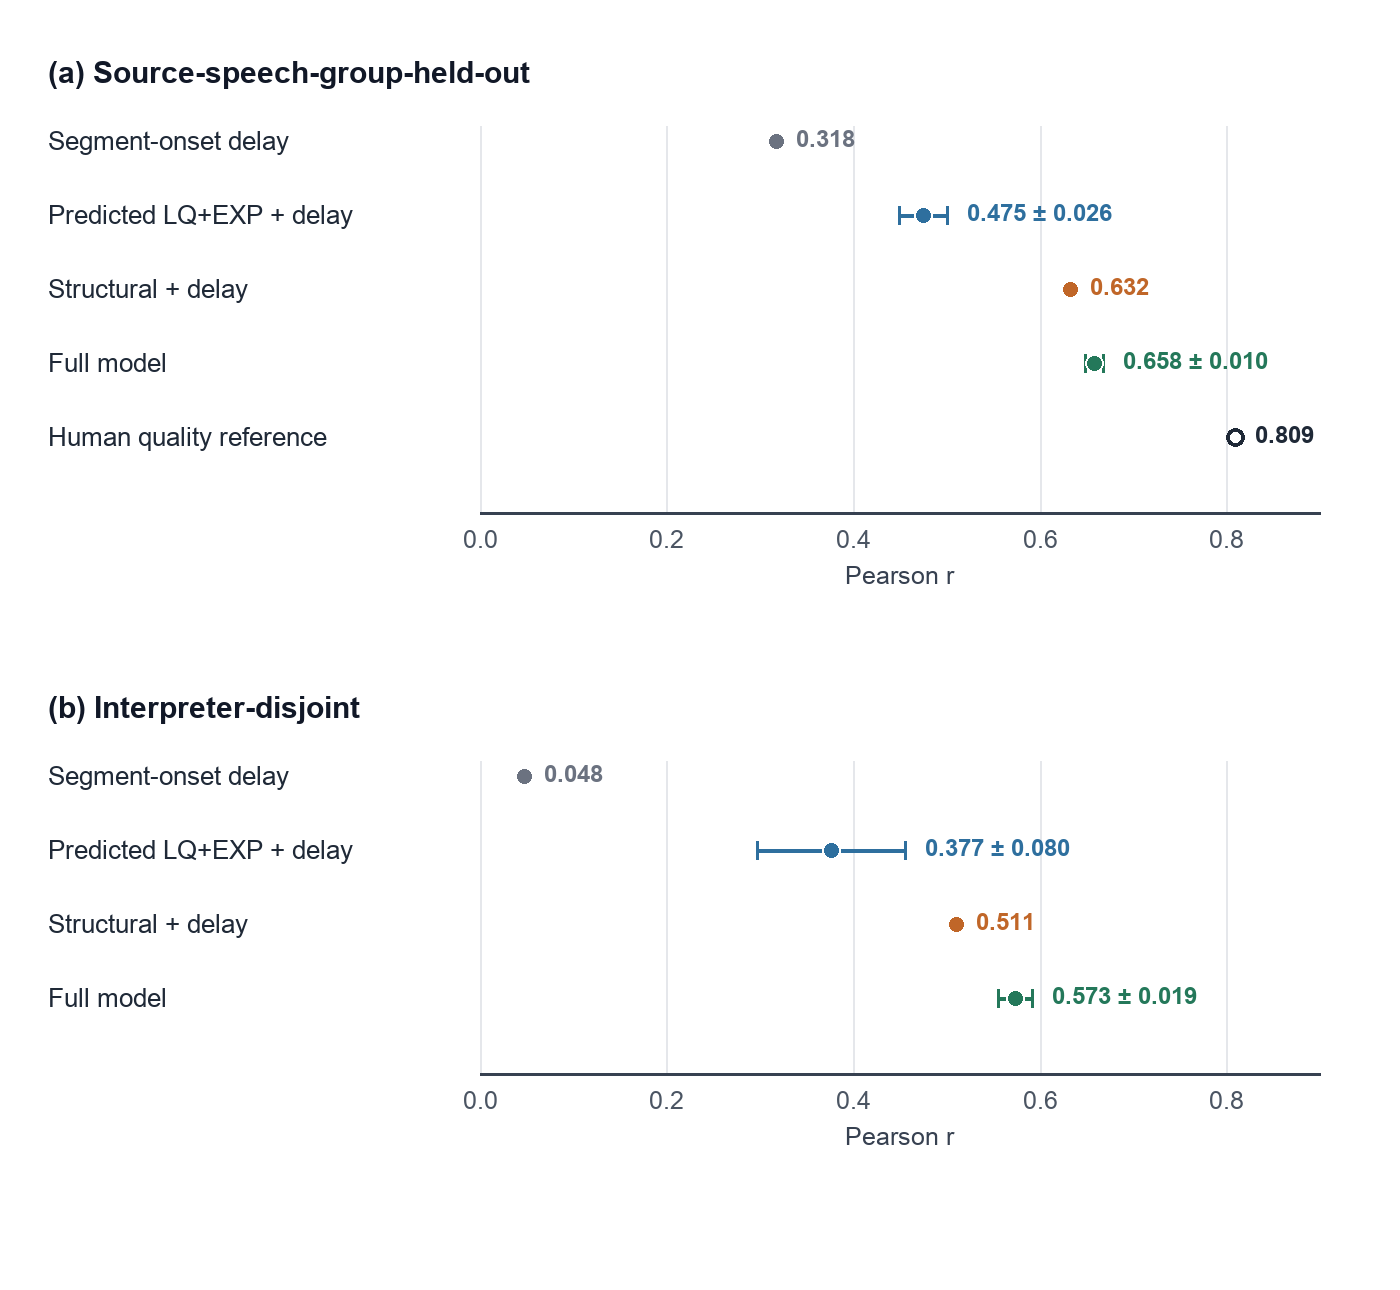
\includegraphics[width=.88\columnwidth]{figures/fig_main_model_comparison.png}
\caption{Main Pearson $r$ comparison. Automatic-row error bars are sample SD across three fixed seeds; clustered CIs appear in text. Deterministic systems appear once, and the hollow marker is the same-rubric human-quality reference.}
\label{fig:main-comparison}
\end{figure}

\subsection{Aggregate-Target Main Results}
\begin{table*}[t]
\centering
\scriptsize
\caption{Source-speech-group-held-out prediction of the predefined two-rater professional aggregate. Automatic rows are mean $\pm$ seed SD; the final row is the same-rubric human-quality reference.}
\label{tab:main}
\begin{tabular}{lccc}
\toprule
System & Pearson $r$ & Spearman $r_S$ & MSE \\
\midrule
Segment-onset delay only & \DelayPearson & \DelaySpearman & \DelayMSE \\
Predicted LQ+EXP & $\QualityPearson\pm\QualityPearsonSD$ & $\QualitySpearman\pm\QualitySpearmanSD$ & $\QualityMSE\pm\QualityMSESD$ \\
Predicted LQ+EXP + delay & $\QualityDelayPearson\pm\QualityDelayPearsonSD$ & $\QualityDelaySpearman\pm\QualityDelaySpearmanSD$ & $\QualityDelayMSE\pm\QualityDelayMSESD$ \\
Lexical/structural + delay & \StructureDelayPearson & \StructureDelaySpearman & \StructureDelayMSE \\
Predicted LQ+EXP + structural + delay & $\mathbf{\FullPearson\pm\FullPearsonSD}$ & $\mathbf{\FullSpearman\pm\FullSpearmanSD}$ & $\mathbf{\FullMSE\pm\FullMSESD}$ \\
\midrule
Same-rubric human-quality reference & \HumanPearson & \HumanSpearman & \HumanMSE \\
\bottomrule
\end{tabular}
\end{table*}

Table~\ref{tab:main} and Figure~\ref{fig:main-comparison} show that delay reaches $r=\DelayPearson$, predicted LQ+EXP $\QualityPearson\pm\QualityPearsonSD$, and predicted quality+delay $\QualityDelayPearson\pm\QualityDelayPearsonSD$. The primary prespecified comparison favors quality+delay over timing-only ($\Delta r=\PrimaryDeltaPearson$, two-sided exact whole-speech-group swap $p=\PrimaryPValue$) and addresses whether professionally supervised quality signals add information absent from onset timing. It does not establish the neural system as the strongest deployable text model: structural+delay reaches $\StructureDelayPearson$, while the full model reaches $\FullPearson\pm\FullPearsonSD$, with $\Delta r=\SecondaryDeltaPearson$ [$\SecondaryDeltaPearsonCILow,\SecondaryDeltaPearsonCIHigh$] and $\Delta\mathrm{MSE}=\SecondaryDeltaMSE$ [$\SecondaryDeltaMSECILow,\SecondaryDeltaMSECIHigh$]. Seed- and group-level effects are positive but heterogeneous; Appendix~B reports their distribution.

\paragraph{Speech-group-clustered uncertainty.} In \BootstrapDraws\ draws that resample the \SpeechGroupN\ speech groups with replacement and retain all segments in each selected group, quality+delay obtains $r=\QualityDelayPearson$ [$\QualityDelayPearsonCILow,\QualityDelayPearsonCIHigh$], $r_S=\QualityDelaySpearman$ [$\QualityDelaySpearmanCILow,\QualityDelaySpearmanCIHigh$], MSE $\QualityDelayMSE$ [$\QualityDelayMSECILow,\QualityDelayMSECIHigh$], and MAE $\QualityDelayMAE$ [$\QualityDelayMAECILow,\QualityDelayMAECIHigh$]. Relative to timing-only, $\Delta r=\PrimaryBootstrapDeltaPearson$ [$\PrimaryBootstrapDeltaPearsonCILow,\PrimaryBootstrapDeltaPearsonCIHigh$], $\Delta r_S=\PrimaryBootstrapDeltaSpearman$ [$\PrimaryBootstrapDeltaSpearmanCILow,\PrimaryBootstrapDeltaSpearmanCIHigh$], $\Delta$MSE $=\PrimaryBootstrapDeltaMSE$ [$\PrimaryBootstrapDeltaMSECILow,\PrimaryBootstrapDeltaMSECIHigh$], and $\Delta$MAE $=\PrimaryBootstrapDeltaMAE$ [$\PrimaryBootstrapDeltaMAECILow,\PrimaryBootstrapDeltaMAECIHigh$]. Its smaller gain over predicted quality is $\Delta r=\QualityAddedDelayDeltaPearson$ [$\QualityAddedDelayDeltaPearsonCILow,\QualityAddedDelayDeltaPearsonCIHigh$]. The $\pm$ values remain fixed-seed SDs.

\paragraph{Range sensitivity.} Raw quality+delay Ridge has no predictions below .5 and $\SourceUpperViolationMean/\CohortN$ ($\SourceUpperViolationPercent\%$) above 3.0. Clipping preserves performance ($r=\SourceClippedPearson\pm\SourceClippedPearsonSD$), while a fold-trained bounded model retains $r=\SourceBoundedPearson\pm\SourceBoundedPearsonSD$. Interpreter-disjoint clipping changes $r$ only from $\LOIOQualityDelayPearson\pm\LOIOQualityDelayPearsonSD$ to $\LOIOClippedPearson\pm\LOIOClippedPearsonSD$; Appendix~B reports full range, error, and calibration results.

\subsection{Structural-versus-Neural Signal Analysis}
Structural features explain limited variation in predicted quality (held-out $R^2=\ResidualLQLow$--$\ResidualLQHigh$ for LQ and $\ResidualEXPLow$--$\ResidualEXPHigh$ for EXP). Low structure-to-quality $R^2$ does not imply that raw quality contributes an orthogonal promptness signal: with both feature families in the linear second stage, residualization can preserve nearly the same joint prediction space. Residualized quality alone is weak ($r=\ResidualOnlyPearsonLow$--$\ResidualOnlyPearsonHigh$), promptness-residual prediction yields partial $R^2=\ResidualPartialRLow$--$\ResidualPartialRHigh$, and all seed-specific $\Delta r$ intervals cross zero. Accordingly, we interpret this comparison as a representation audit rather than an independent quality effect; Appendix~B gives details.

\subsection{Cross-Rater Analysis}
Using human LQ/EXP under the same held-out folds, R05 and R06 promptness ratings have Pearson $\InterraterPearson$ and ICC$(2,1)=\InterraterICC$; Appendix~B gives the full reliability audit.

With delay included, same-rater associations are $r=\CrossRtoR$ for R05 and $\CrossStoS$ for R06; cross-rater associations are $\CrossRtoS$ (R05 quality$\rightarrow$R06 promptness) and $\CrossStoR$ in reverse (Appendix Table~\ref{tab:cross-rater}). Under independent blinded scoring, these associations cannot arise from direct score sharing. They indicate cross-evaluator commonality in the quality--promptness relationship, but their asymmetry shows strong calibration dependence. Common rubric order and same-session scoring may still create parallel halo and anchoring effects.

\subsection{Interpreter-Disjoint Results}
After each interpreter is excluded, predicted quality+delay reaches pooled $r=\LOIOQualityDelayPearson\pm\LOIOQualityDelayPearsonSD$ versus \LOIODelayPearson\ for timing-only; structural+delay reaches \LOIOStructureDelayPearson\ and the full model $\LOIOFullPearson\pm\LOIOFullPearsonSD$ (Appendix Table~\ref{tab:loio}). The full model retains centered $r=\LOIOFullCenteredPearson\pm\LOIOFullCenteredPearsonSD$ and macro $r=\LOIOFullMacroPearson\pm\LOIOFullMacroPearsonSD$, but performance varies across interpreters. Source speeches may recur in this protocol.

\subsection{Direction Audit}
Direction-specific results are descriptive because the cohort contains 505 Chinese-to-English but only 117 English-to-Chinese segments. The full model is positive in both directions; Appendix Table~\ref{tab:automatic-direction} reports the automatic systems, and Appendix~B gives human-label sensitivity.
